To address these complications in practice, a preliminary exercise was carried out which aimed to characterise the expected initial and final state interactions for the observation of a CC0\(\pi\) event in SBND. Alongside this, the potential backgrounds were also categorised in order to quantify their effect. 

    This exercise also contributed to the initial construction of an anaylsis framework which will eventually be expanded to incorporate fully reconstructed simulations and multiple final state topologies. In the first stage of this exercise however, a MC sample of neutrino events was generated and a manual amount of smearing was applied to them along with energy cuts and an application of pionic impurities in order to loosely represent reconstructed events in SBND whilst training the analysis framework.  

\subsection{Smearing}

The Monte Carlo sample of SBND events was simulated using the Default+MEC GENIE model and the SBND flux, given in Figure~\ref{fig:SBNDFlux}. The quantites applied to the smearing, impurity additions and energy cuts are as follows \footnotemark,

\footnotetext{these quantities are in no way physically motivated. This entire anaylsis will eventually be implemented in a software framework which provides a dedicated reconstruction for liquid argon and so the smearing will not be a necessary step.}

    \begin{figure}[h!]
        \centering
        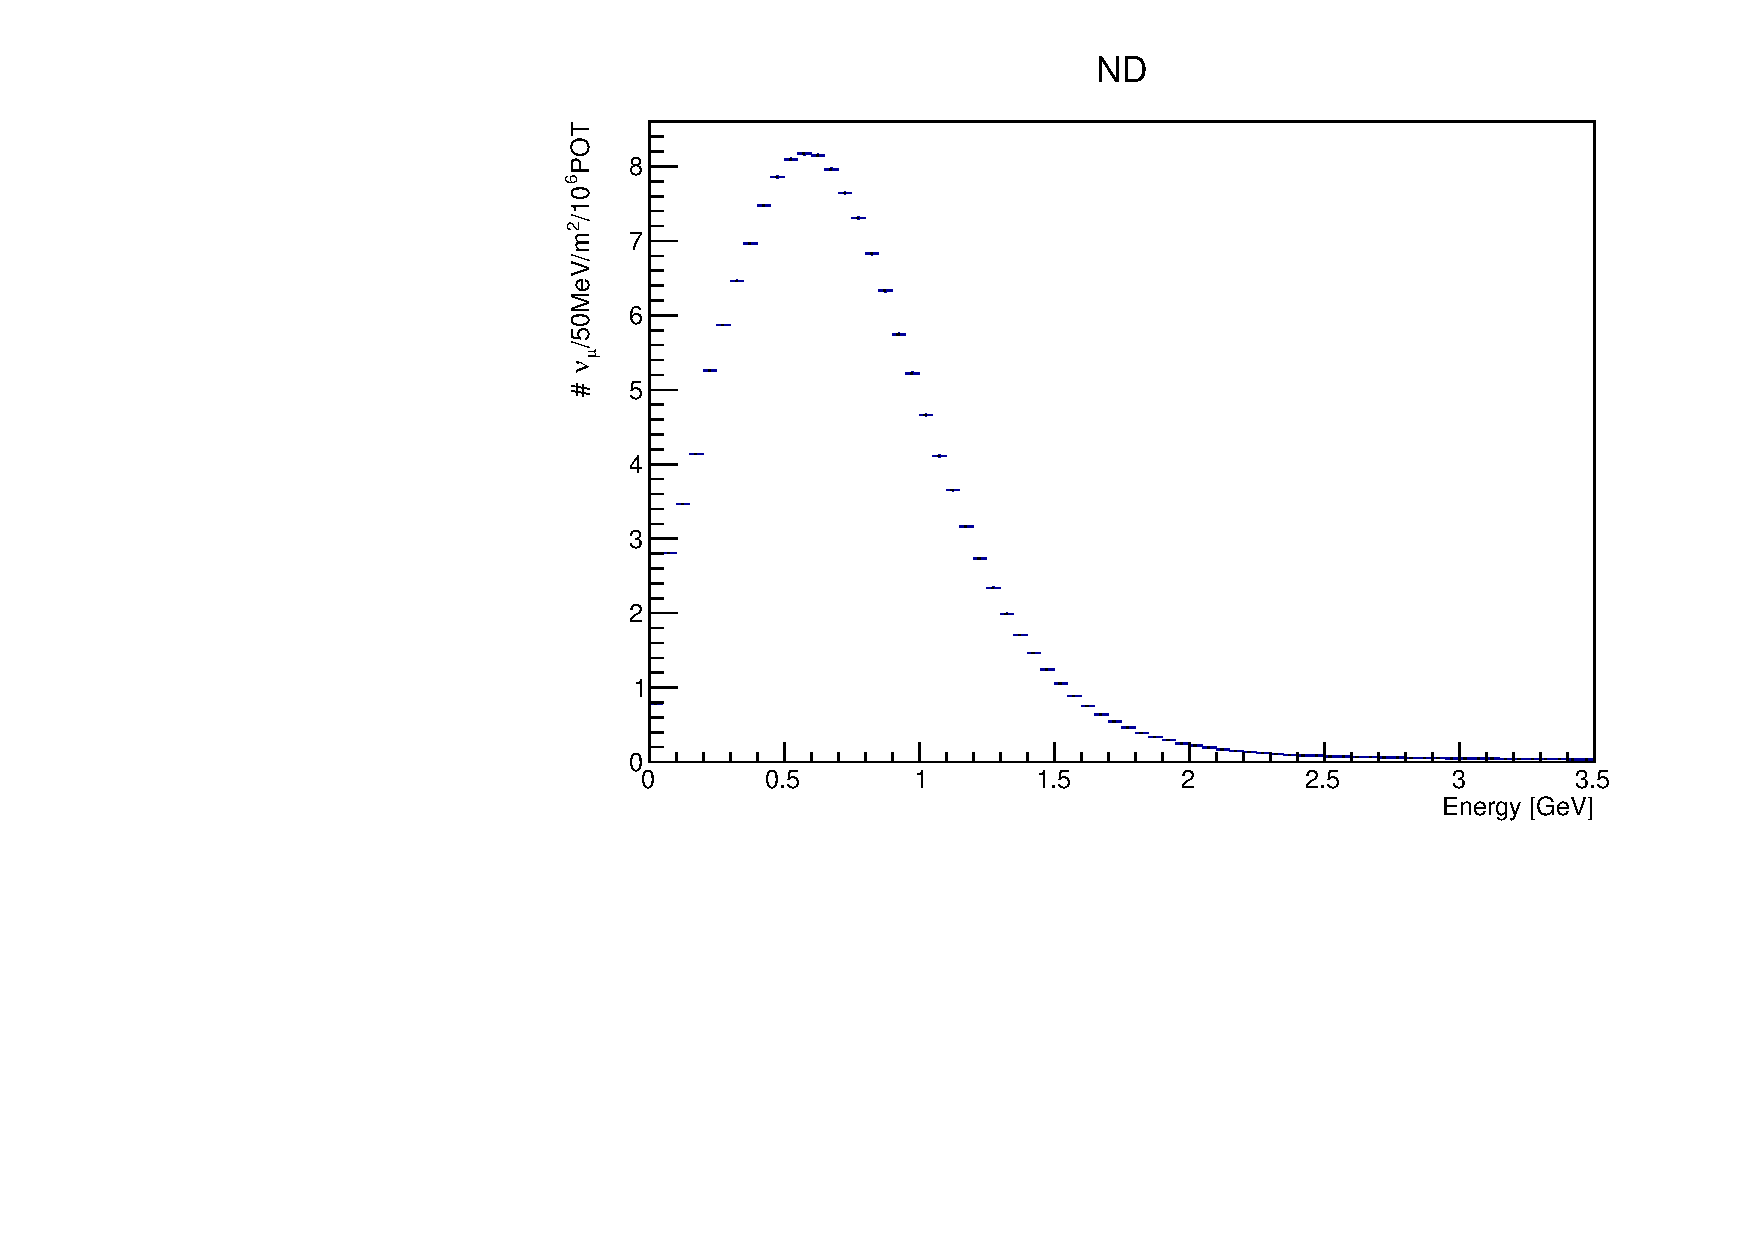
\includegraphics[width=.8\textwidth, trim=0 0 0 1cm, clip]{images/sbnd_flux.pdf}
        \caption{The flux of \(\nu_{\mu}\) at the short baseline near detector used to generate the neutrino events used throughout the following exercise}
        \label{fig:SBNDFlux}
    \end{figure}

\begin{itemize}
    \setlength\itemsep{.5em}
    \item Kinetic energy of the \(\mu\) : 10\%
    \item Opening angle of the \(\mu\) : 5\(^{\circ}\)
    \item \(\mu\) kinetic energy threshold > 50 MeV
    \item \(\pi^{\pm}\) kinetic energy threshold > 50 MeV
    \item Proton kinetic energy threshold > 50 MeV
    \item NC \(\pi^{\pm} \Leftrightarrow \mu\) mixup : 20\% of \(\pi^{\pm}\)
\end{itemize}

To smear the angular quantities, a random point was chosen from a Gaussian distribution about the true angle with a standard deviation of 5\(^{\circ}\). Since the cosine of this angle was the variable of interest, if the smeared angle was below 0\(^{\circ}\) the cosine of such a value would still be physically viable. However, a value of kinetic energy below 0 is not physically possible - since this implies the outgoing particles are travelling in the reverse direction to an interaction which occurred between a forward-going neutrino and a stationary nucleon. In this case, a lognormal distribution was used to randomly generate a kinetic energy with the true value as the mean, and a standard deviation of 10\%. 

The definition of a point on a lognormal distribution is given by equations~(\ref{eq:lognorm}), (\ref{eq:lognorm1}) and~(\ref{eq:lognorm2}) and is shown entirely generally for 100,000 data points about a mean of 10 and a variance of 0.5 in Figure~\ref{fig:logNorm}.

    \begin{equation}\label{eq:lognorm}
        X = e^{(\mu + \sigma)}
    \end{equation}

    \begin{equation}\label{eq:lognorm1}
        \mu = \ln \left( \frac{m}{\sqrt{1 + \frac{v}{m^2}}} \right)
    \end{equation}

    \begin{equation}\label{eq:lognorm2}
        \sigma = \sqrt{\ln \left( 1 + \frac{v}{m^2} \right) }
    \end{equation}
    
    where \( m \) is the mean, \( v \) is the variance or standard deviation squared and X is the smeared data point.   

    \begin{figure}[h!]
        \centering
        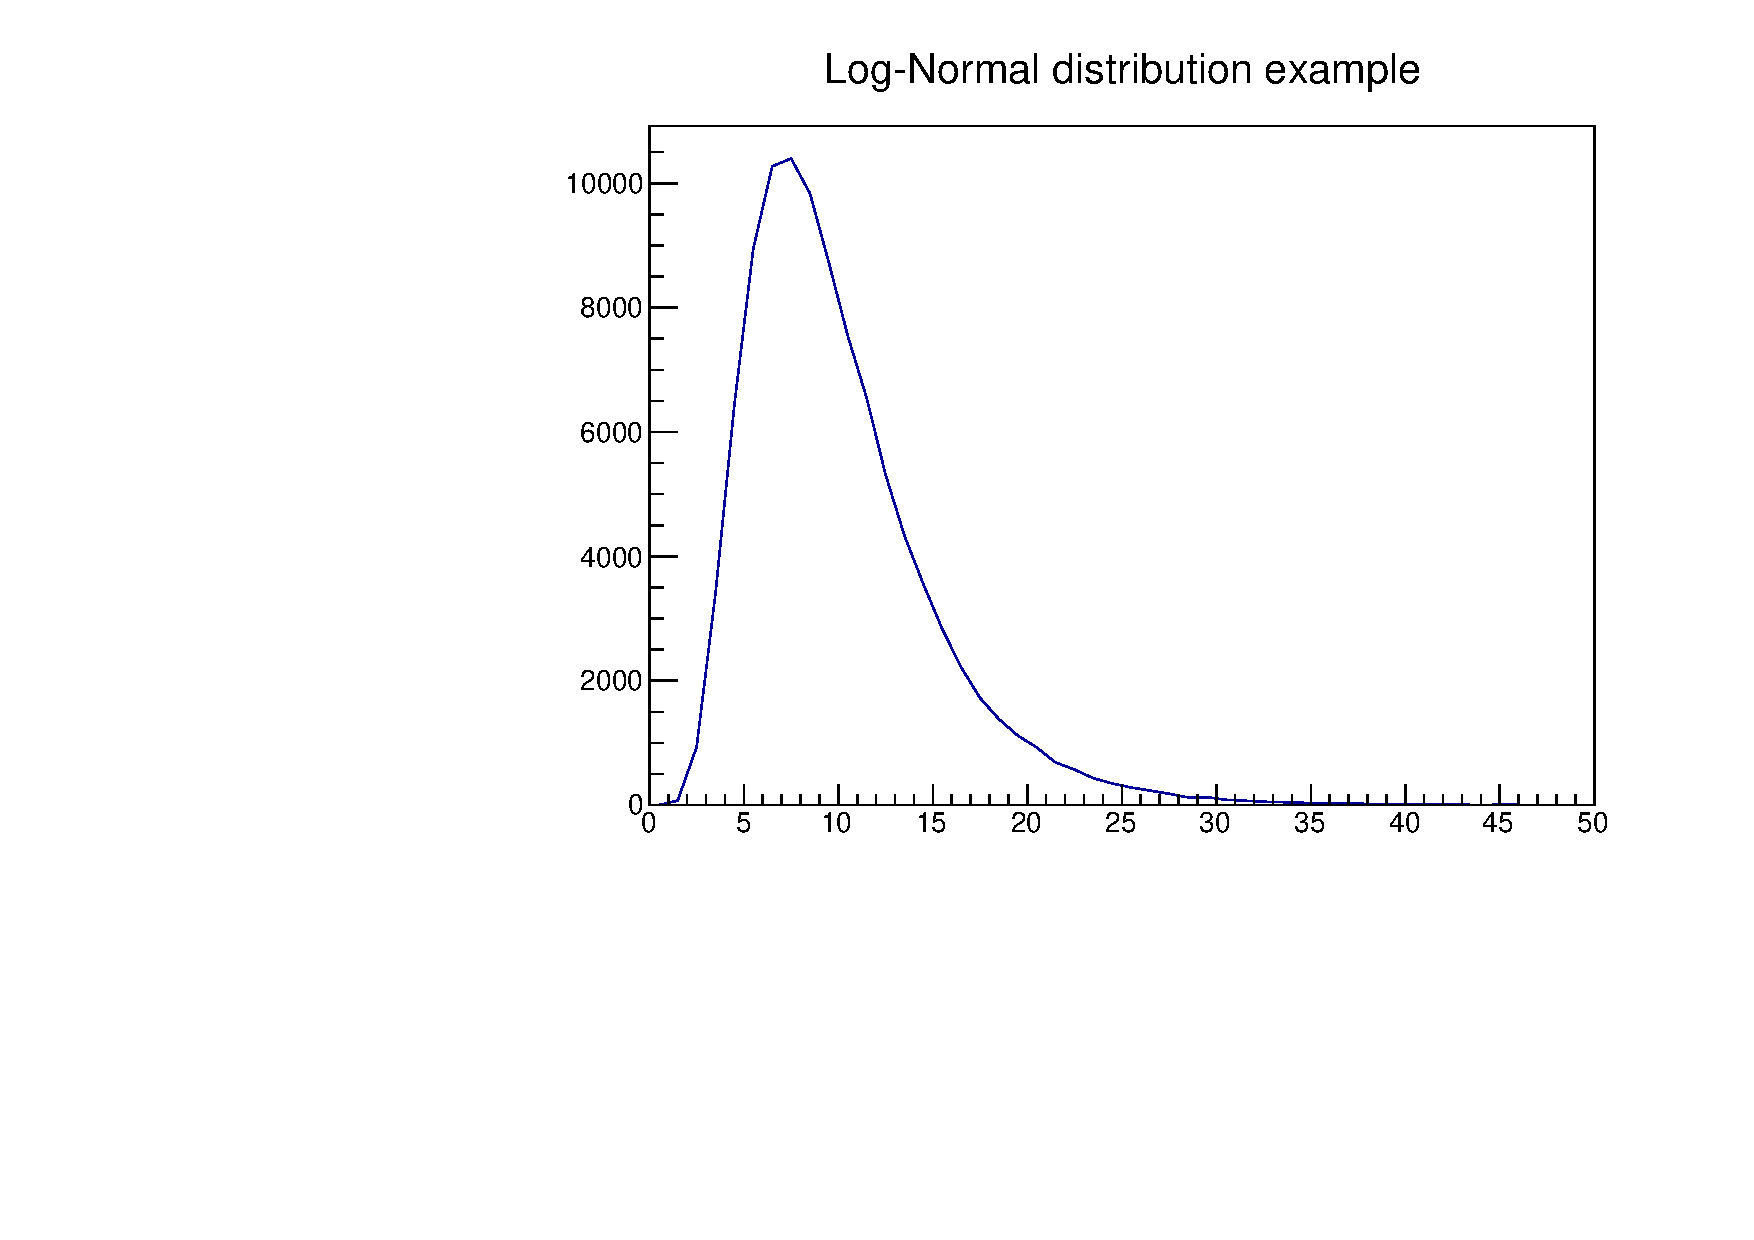
\includegraphics[width=.8\textwidth, trim=0 0 0 1cm, clip]{images/log_norm.pdf}
        \caption{An entirely general lognormal distribution, this is used to calculate smeared kinetic energies because the points never go below 0. T < 0 MeV is an unphysical value in a detector which accepts a forward-going neutrino beam.}
        \label{fig:logNorm}
    \end{figure}

In a CC0\(\pi\) interaction, the potential backgrounds within the detector will contaminate the signal for various reasons, including:

\begin{itemize}
    \item Low energy energy depositions of pions
    \item Mis-identification of pions
    \item ...
\end{itemize}

In this exercise, both the signal and background were split into potential contributing topologies in order to highlight the interaction characteristics within the detector and identify the channels which will be of interest in SBND. 

\subsection{Pre-FSI categorisation}

Using MC information, it is possible to characterise the signal based on the true, interaction-level event topology. Reconstruction within a detector would not allow for this, but studying these distributions gives and idea of how frequently pions get absorbed and other internucleon interactions take place.  




\subsection{Post-FSI categorisation}

The following results are the characterised signal and background for CC0\(\pi\) in SBND split into different event topologies. 

\subsection{Moving forwards}

One potential extention to this exercise would be to compare the smeared/reconstructed predictions with existing data to draw comparisons in a more realistic situation. The chosen experiment for this is MiniBooNE, which had the same baseline and energy range as SBND will have. For this reason, the kinematics studied were the same as that of MiniBooNE: muon kinetic energy as a function of the opening angle of the final state particles. An example comparison between
MiniBooNE data and predictions made by GENIE is shown in Figure~\ref{fig:MBComp}. The binning was also replicated in this exercise for the same reasons.

    % Plan
    \begin{itemize}
        \item RESULTS
        \item This will be better implemented in LArSoft using full detector simulation
        \item Efficiency and purity definitions for the detector
    \end{itemize}


\clearpage
